\documentclass[tikz]{standalone}
% Common TikZ styles (built from the user's Graduate Macro Sequence template)
\usepackage{tikz}
\usetikzlibrary{arrows.meta, positioning, calc, decorations.markings}

% Base template styles (user-provided)
\tikzset{
  node style/.style={draw, circle, minimum size=6mm, inner sep=0pt},
  label style/.style={font=\small, sloped, anchor=center},
  arrow style/.style={-{Stealth[length=3mm]}, thick}
}

% Macro-diagram extensions (kept minimal and clean)
\tikzset{
  axis/.style={arrow style},
  curve/.style={thick},
  curve2/.style={thick, dashed},
  helper/.style={thin, dashed},
  dot/.style={circle, fill=black, inner sep=1.2pt},
  lab/.style={font=\small},
  titlelab/.style={font=\small\bfseries},
}

\begin{document}
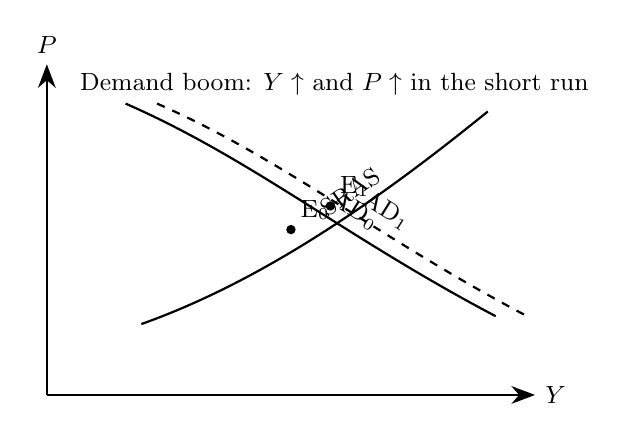
\begin{tikzpicture}[x=1cm,y=1cm]
  \draw[axis] (0,0) -- (6.2,0) node[lab, anchor=west] {$Y$};
  \draw[axis] (0,0) -- (0,4.2) node[lab, anchor=south] {$P$};

  \draw[curve] (1.0,3.7) .. controls (2.6,3.0) and (3.8,2.0) .. (5.7,1.0)
    node[label style, pos=0.62, above] {AD$_0$};

  \draw[curve2] (1.4,3.7) .. controls (3.0,3.0) and (4.2,2.0) .. (6.1,1.0)
    node[label style, pos=0.62, above] {AD$_1$};

  \draw[curve] (1.2,0.9) .. controls (2.6,1.4) and (4.0,2.3) .. (5.6,3.6)
    node[label style, pos=0.65, above] {SRAS};

  \node[dot] (E0) at (3.1,2.1) {};
  \node[dot] (E1) at (3.6,2.4) {};
  \node[lab, anchor=south west] at (E0) {E$_0$};
  \node[lab, anchor=south west] at (E1) {E$_1$};

  \node[lab, anchor=west] at (0.3,3.95) {Demand boom: $Y\uparrow$ and $P\uparrow$ in the short run};
\end{tikzpicture}
\end{document}
